\chapter{Physical Properties of CO emitters}

\section{Wide ASPECS}

Wide ASPECS builds upon the Pilot and Large Program, going much wider, but also shallower. This means that Wide ASPECS cannot capture as dim CO emitters, but because of the much larger cosmic volume looked at, it can find rarer, but very bright CO emitters that did not happen to fall within the Large Program and Pilot survey bounds.

The data for this survey was observed in ALMA Cycle 5 and was observed in Band 3 (3mm) for ~20 hours in 130 pointings and three frequency settings. The three frequency settings A, B, and C each have an upper side band and a lower side band, as shown in Fig. \ref{fig:ASPECS_Freq}. The lower side bands covered 91.704-95.446 GHz, 84.209-87.951 GHz, and 87.954-91.696 GHz for A, B, and C settings respectively. The upper side bands covered the frequency ranges 103.704-107.446 GHz, 96.209-99.951 GHz, and 99.954-103.696 GHz for A, B, and C settings respectively. The survey covered ~52.5 arcminutes$^2$ of the sky at 20\% sensitivity, and ~43 arcminutes$^2$ at 50\% sensitivity. This means Wide ASPECS covers roughly five times the area of the ASPECS Large Program. The sensitivity of the survey reaches $\sim$0.9 mJy beam$^{-1}$ per 24.4 kms$^{-1}$ channel. This raw data was processed with the CASA ALMA pipeline into six data cubes, one for each upper side band and lower side band of the three frequency settings.

\begin{figure}[!htbp]
\centering 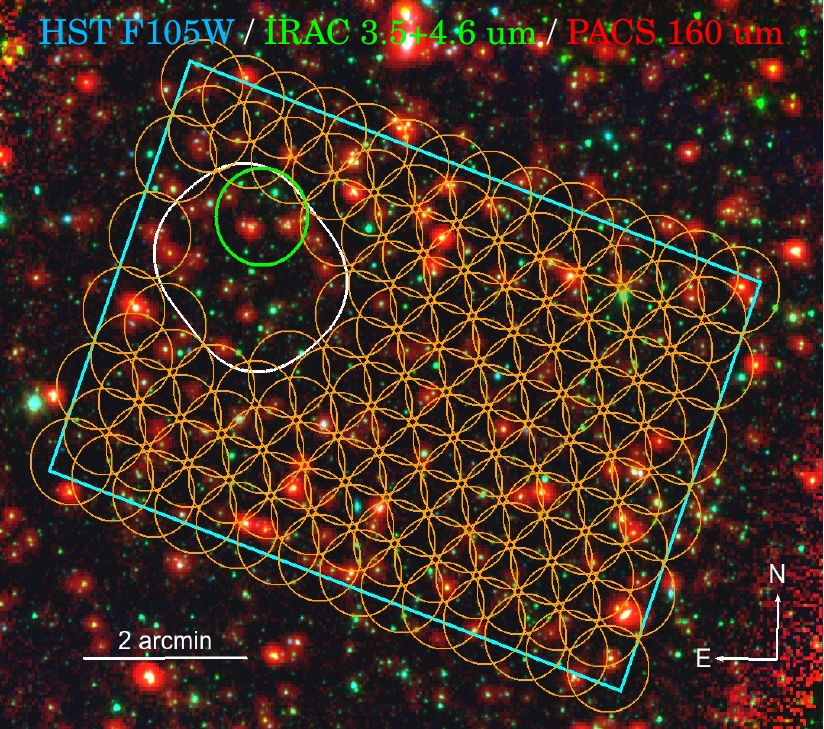
\includegraphics[width=120mm]{Wide_ASPECS_Coverage.png}
\caption{Spatial coverage of ASPECS Pilot (Green), Large Program (White), and Wide (Yellow) showing each of the individual pointings. The area covered by the Pilot is $~$1 arcmin$^2$, by the Large Program $~$5 arcmin$^2$, and by Wide ASPECS, $~$52.5 armin$^2$. The cyan box is the 50\% sensitivity extent of the survey. This region covers the area of the deepest CANDELS observations, where a wealth of ancillary data has been collected in over 30 photometric bands. Figure adapted from Decarli et al. (in prep.)} % Decarli in report
% Put this in the Wide ASPECS description stuff
\label{fig:ASPECS_Coverage}
\end{figure}

\begin{figure}[!htbp]
\centering
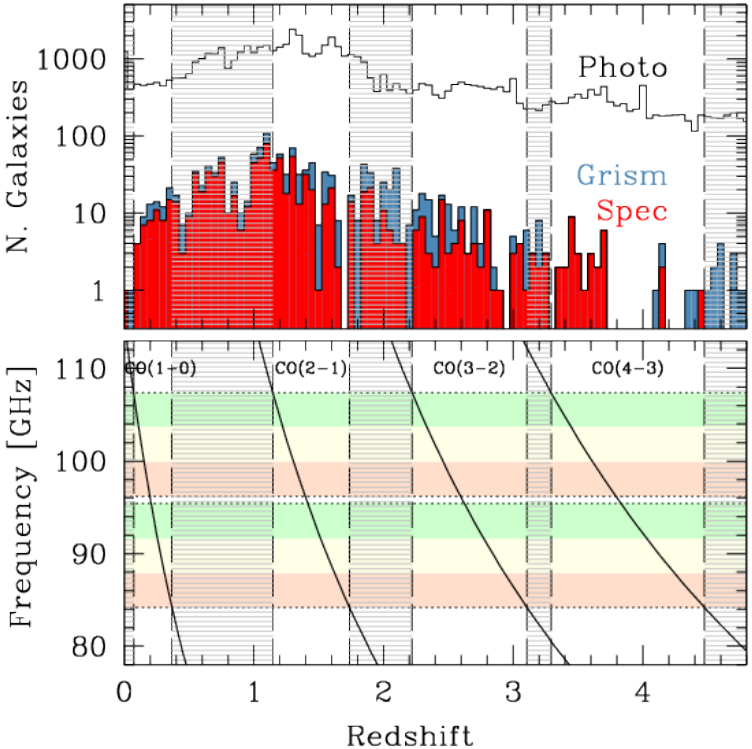
\includegraphics[width=120mm]{Wide_ASPECS_Freq.png}
\caption{Spectral and redshift coverage of Wide ASPECS in relation to the redshift distribution of galaxies within the survey field. Wide ASPECS is designed to detect CO line transitions at z$<$0.4, 1.1 $<$ z $<$ 1.8, and 2.2 $<$ z $<$ 4.4. Green, red, and yellow are the frequency ranges for A, B, and C frequency settings respectively. Figure adapted from Decarli et al. (in prep.)}
\label{fig:ASPECS_Freq}
\end{figure}

\begin{table}[!htb]
\caption{Redshift limits and cosmic volume probed for each CO transition observable by Wide ASPECS.}
\begin{tabular}{lllll}\label{table:CO_freq}
Transition & $z_{low}$ & $z_{high}$ & Freq. (GHz) & Volume (Mpc$^3$) \\
\hline
1-0        & 0.0030    & 0.3694     & 115.271     & 4461             \\
2-1        & 1.0059    & 1.7387     & 230.538     & 107411           \\
3-2        & 2.0088    & 3.1080     & 345.796     & 191232           \\
4-3        & 3.0115    & 4.4771     & 461.041     & 237143          
\end{tabular}
\end{table}

\subsection{Ancillary Data}\label{sec:ancillary}

In addition to each of the ALMA data cubes, there is a lot of ancillary data available as the GOODS-South region is one of the most studied regions of the sky. This data has been collected by combining multiple catalogs, first described in \cite{walter2016alma} and expanded with new data in \cite{decarli2019alma}, comprising over 30 photometric bands for over 63000 galaxies in and around the footprint of Wide ASPECS. 26251 galaxies lie within the footprint of Wide ASPECS, of which 2283 have spectroscopic redshifts, and 23968 have photometric redshifts. 

The majority of the ancillary data comes from the Hubble Space Telescope (HST) Cosmic Assembly Near-infrared Deep Extragalactic Legacy Survey (CANDELS)\cite{grogin2011candels, Koekemoer_2011}. Most of the photometric data comes from \cite{skelton20143d}, which additionally includes ground-based optical and NIR photometry from \cite{nonino2009deep, hildebrandt2006gabods, erben2005gabods, retzlaff2010great, Hsieh_2012, 2008ApJ...682..985W, cardamone2010multiwavelength}, as well as Spitzer IRAC 3.6$\mu$m, 4.5$\mu$m, 5.8$\mu$m, and 8.0$\mu$m photometry from \cite{dickinson2003evolution, elbaz2011goods, 2013ApJ...769...80A}. There is also photometric information from the Spitzer MIPS 24$\mu$m from \cite{Whitaker_2014}, and ALMA 1.1mm data from \cite{franco2018goods}. Additional far-infrared data from Herschel PACS at 100$\mu$m and 160$\mu$m as obtained from \cite{elbaz2011goods}. Spectroscopic redshifts came mostly from the MUSE Hubble Ultra Deep Survey \cite{bacon2017, inami2017} while more spectroscopic information was included from \cite{le2005vimos, coe2006galaxies, skelton20143d, morris2015wfc3}. Hubble grism spectroscopy was taken from the 3D-HST survey \cite{momcheva20163d}.

\subsection{Galaxy SED Fitting}

All observations of a galaxy recorded in gamma and X-rays, visible light, infrared, radio and UV give us part of the total spectral energy distribution (SED) of that galaxy. The more wavelengths a galaxy is measured in, the better constrained the SED, and the more complete our understanding of its energy distribution. Software, such as MAGPHYS \cite{da2008simple, da2015alma}, can use these observations to estimate a galaxy's physical parameters. These programs match the observed SED to precomputed models and output likelihood estimates for the properties of a given galaxy, such as the star-formation rate, mass, and dust temperature.

To estimate the properties of the galaxies in the catalog, the SED fitting program MAGPHYS was used \cite{da2008simple, da2015alma}. MAGPHYS computes a marginalized likelihood distribution for each of the different physical parameters of the observed galaxy through comparing the observed SED with the precomputed models. It also outputs the best-fit total SED for a given galaxy. In this report, the MAGPHYS high-z extension was used, which updates the original MAGPHYS with extended star-formation history and dust optical depth priors and adds intergalactic medium absorption in the ultraviolet \cite{da2015alma}.

An example output from MAGPHYS is shown in Fig. \ref{fig:MAGPHYS_Example}, displaying the model, the likelihood values for various physical properties of the galaxy, and the data points used to compute the SED in red. The distribution of the stellar mass, and star-formation rates of all the galaxies fitted with MAGPHYS are shown in Fig. \ref{fig:MAGPHYS_Mstar} and Fig. \ref{fig:MAGPHYS_SFR} respectively. Galaxies whose computed star-formation rate was at or below a $log_{10}(SFR) = -1.99$ were removed from the rest of the analysis, as this seemed to indicate a very poor MAGPHYS fit. That left a total of around 55000 galaxies in the sample, of which 22073 were in the Wide ASPECS footprint.

\begin{figure}[!hbp]
% Make Larger
\centering 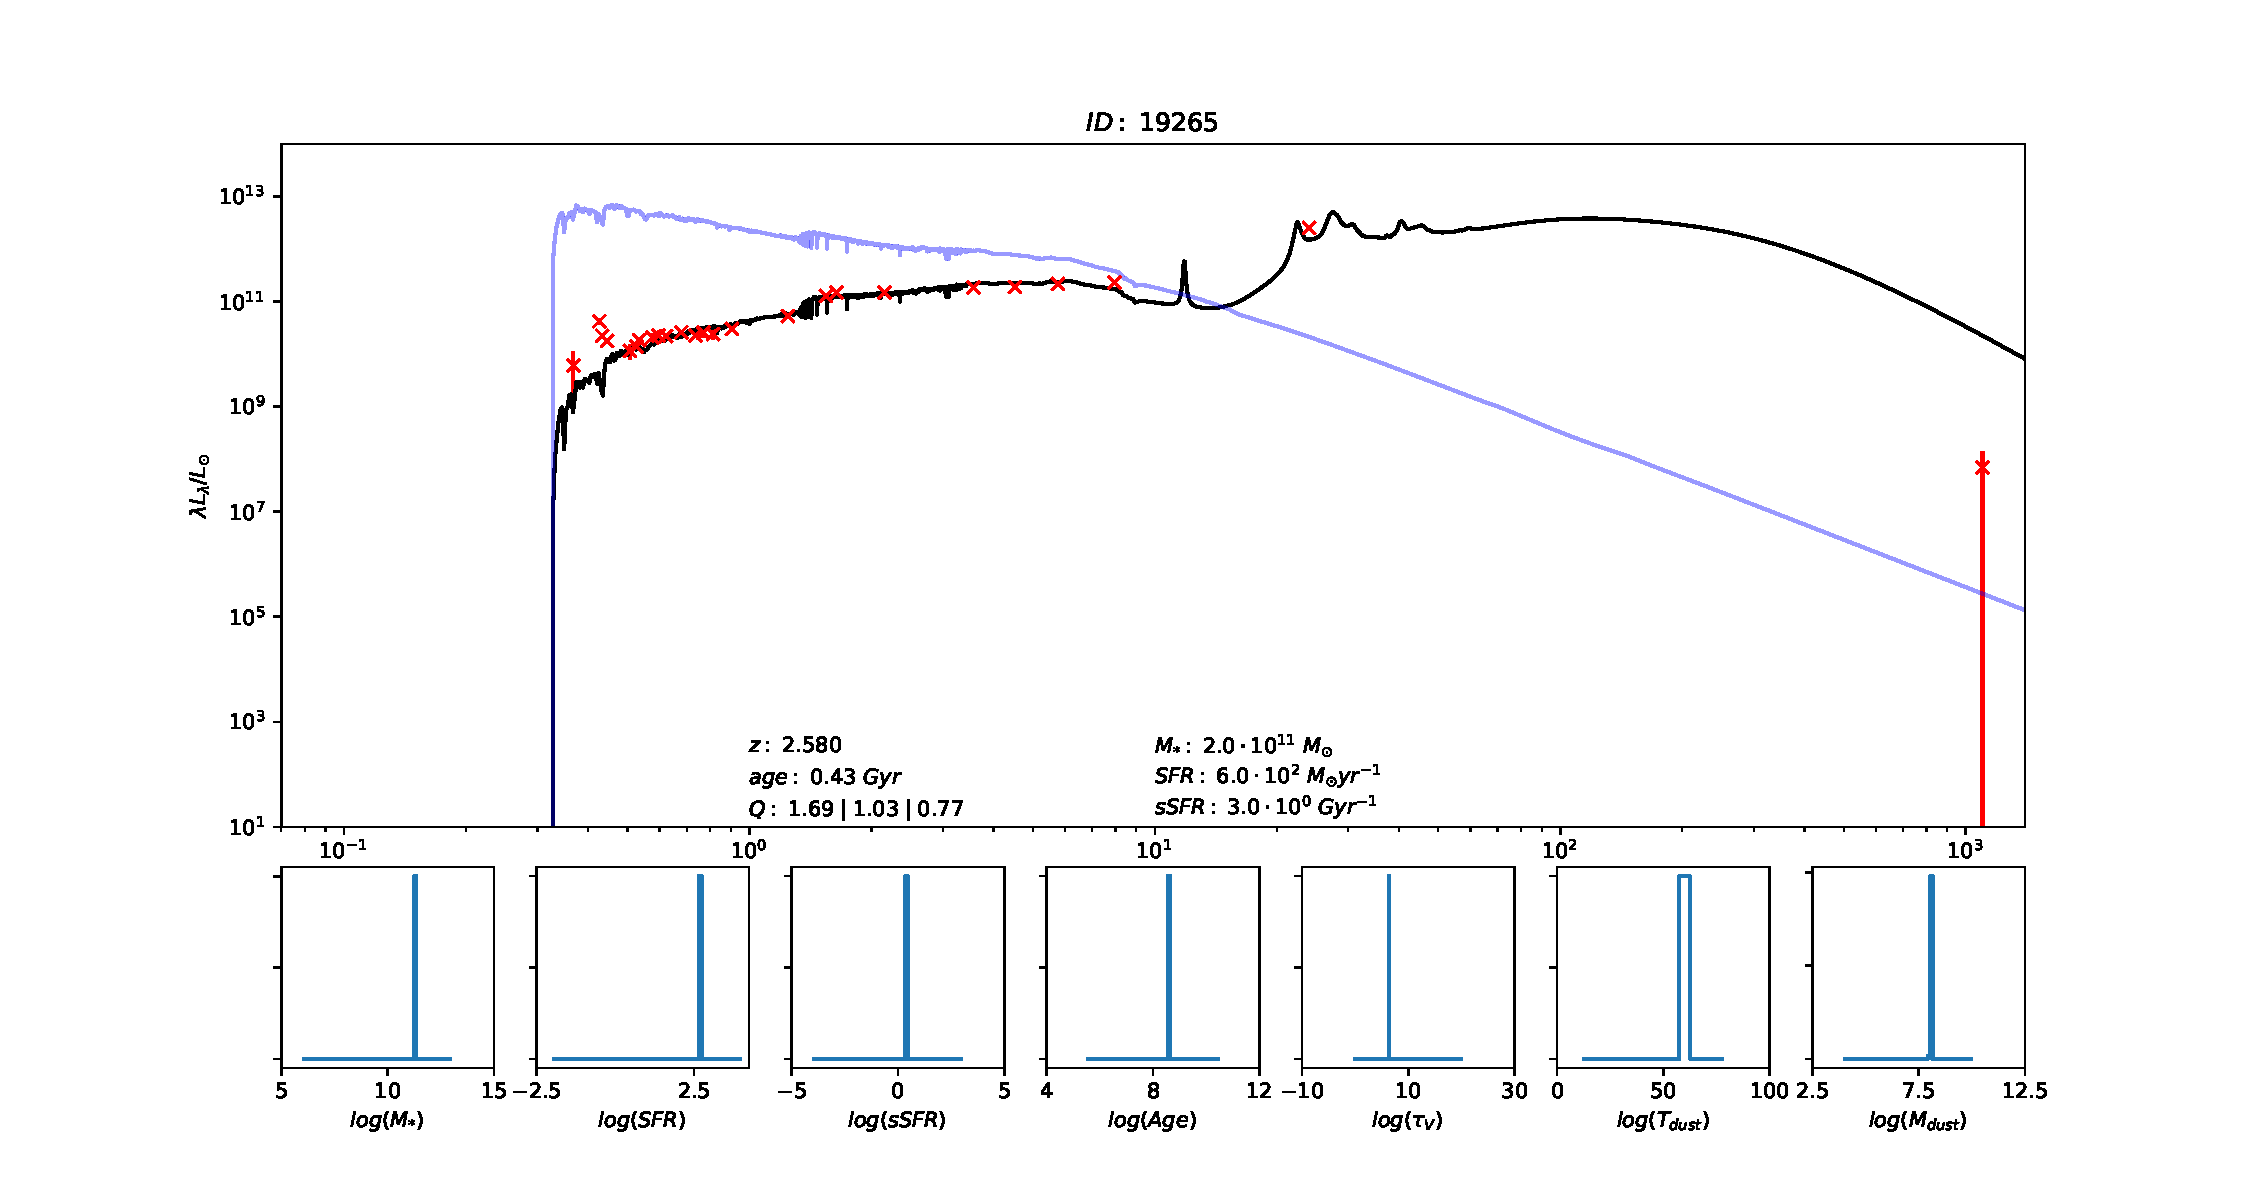
\includegraphics[width=160mm]{19265.pdf}
\caption{Example MAGPHYS output, from the most massive matched galaxy, ID.1 in Table \ref{table:Catalog}. The blue line is the spectrum of the galaxy without attenuation. The black line is the model used by MAGPHYS. The red dots are the data points. The bottom row of graphs show the probability distribution for various physical properties.}
\label{fig:MAGPHYS_Example}
\end{figure}

\begin{figure}[!htbp]
\centering 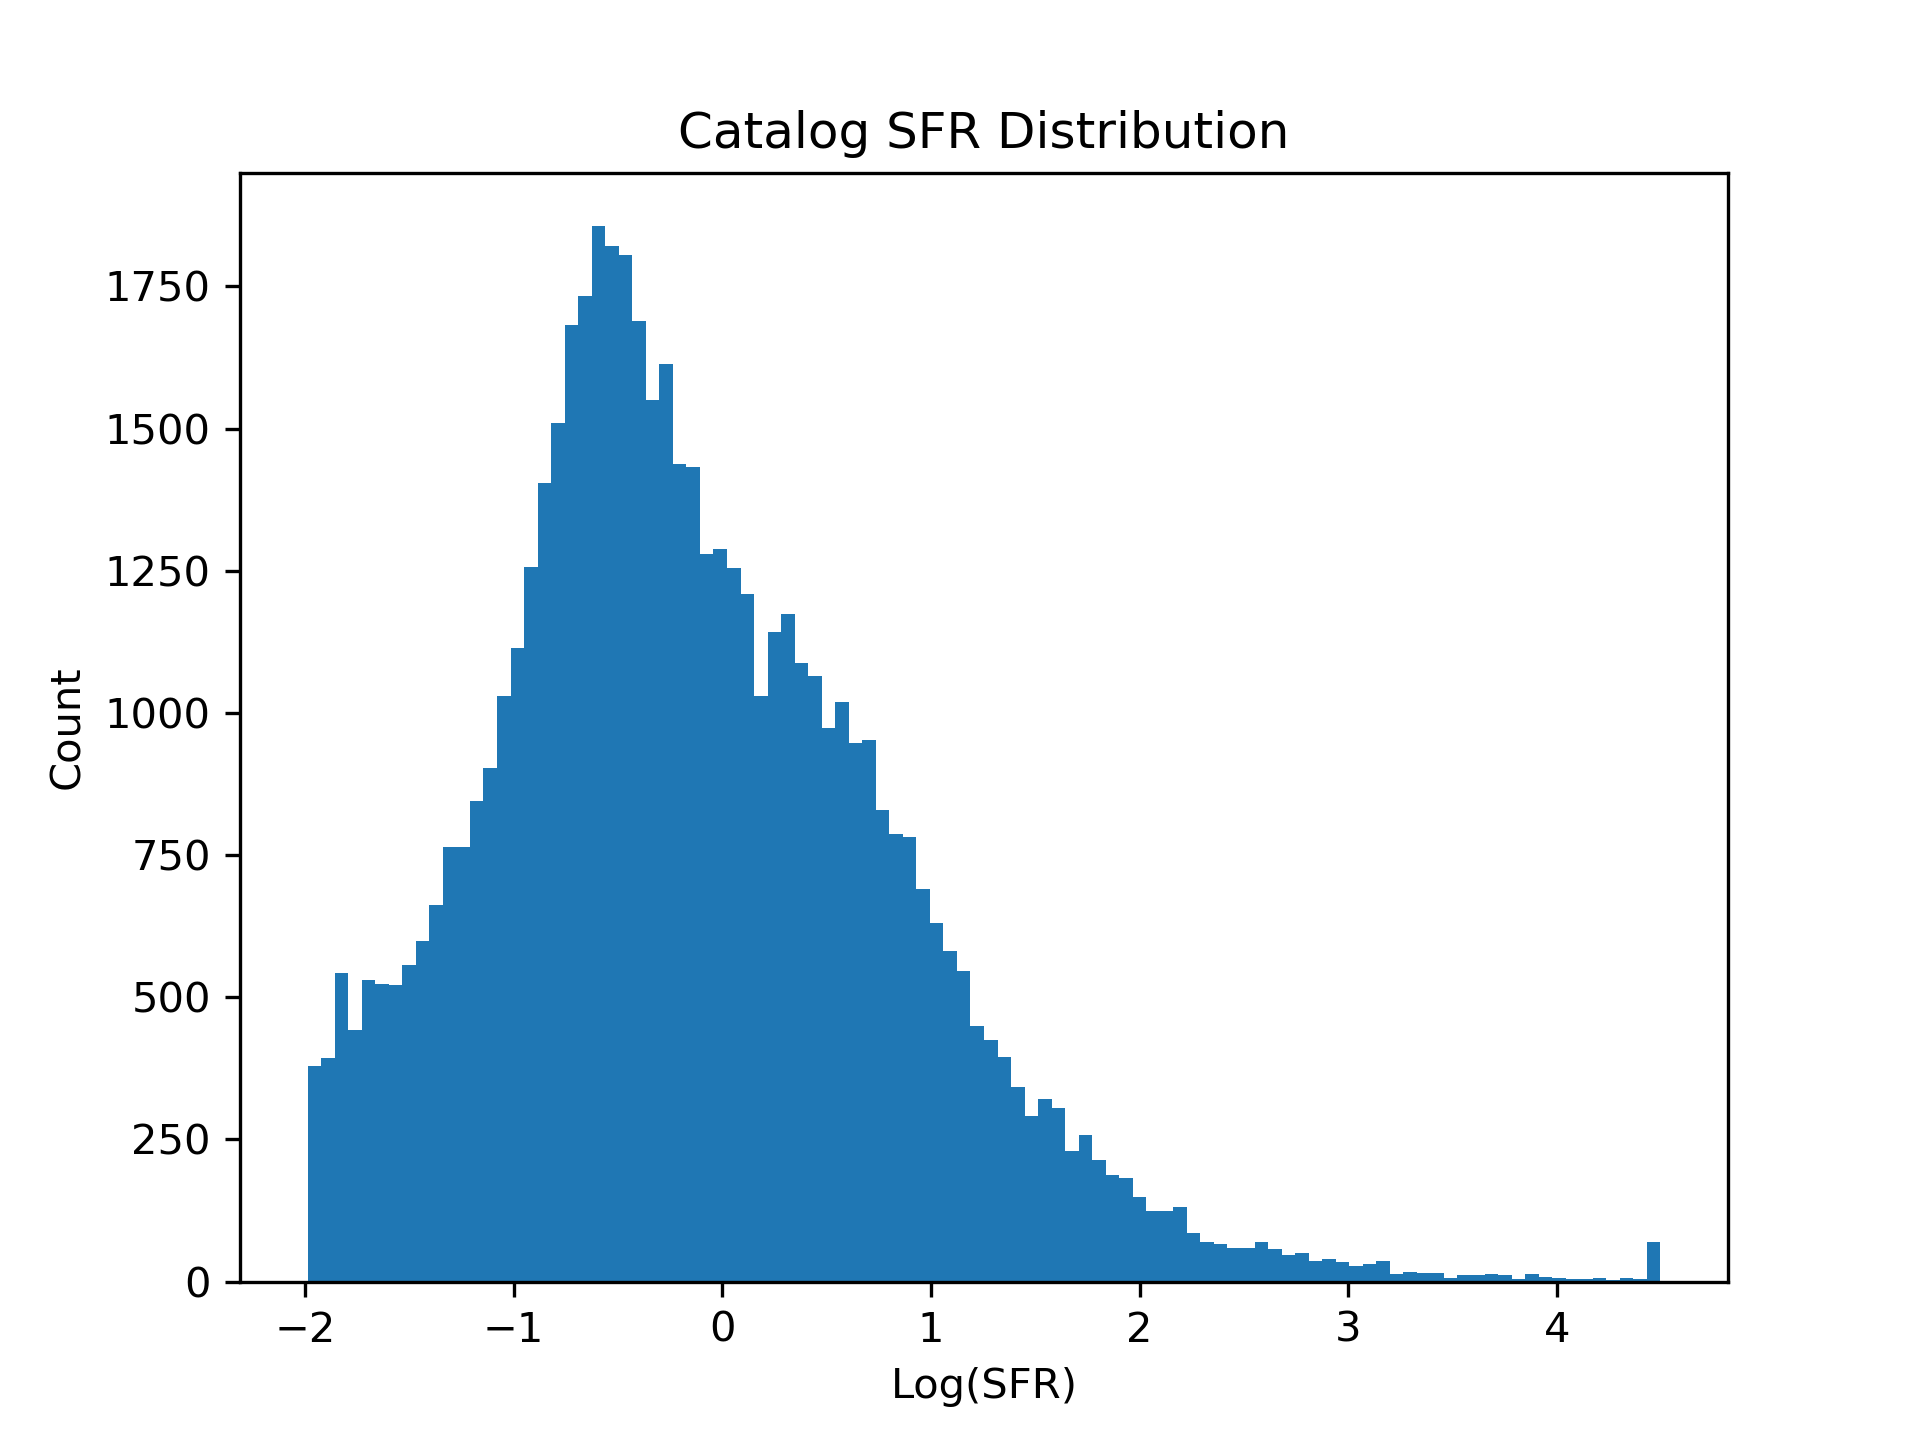
\includegraphics[width=87mm]{Survey/MAGPHYS_SFR.png}
\caption{Distribution of star-formation rate for all galaxies in the catalog. The cutoff at -1.99 is from the quality cut to remove galaxies that had very poor MAGPHYS fits.}
\label{fig:MAGPHYS_SFR}
\end{figure}

\begin{figure}[!htbp]
\centering 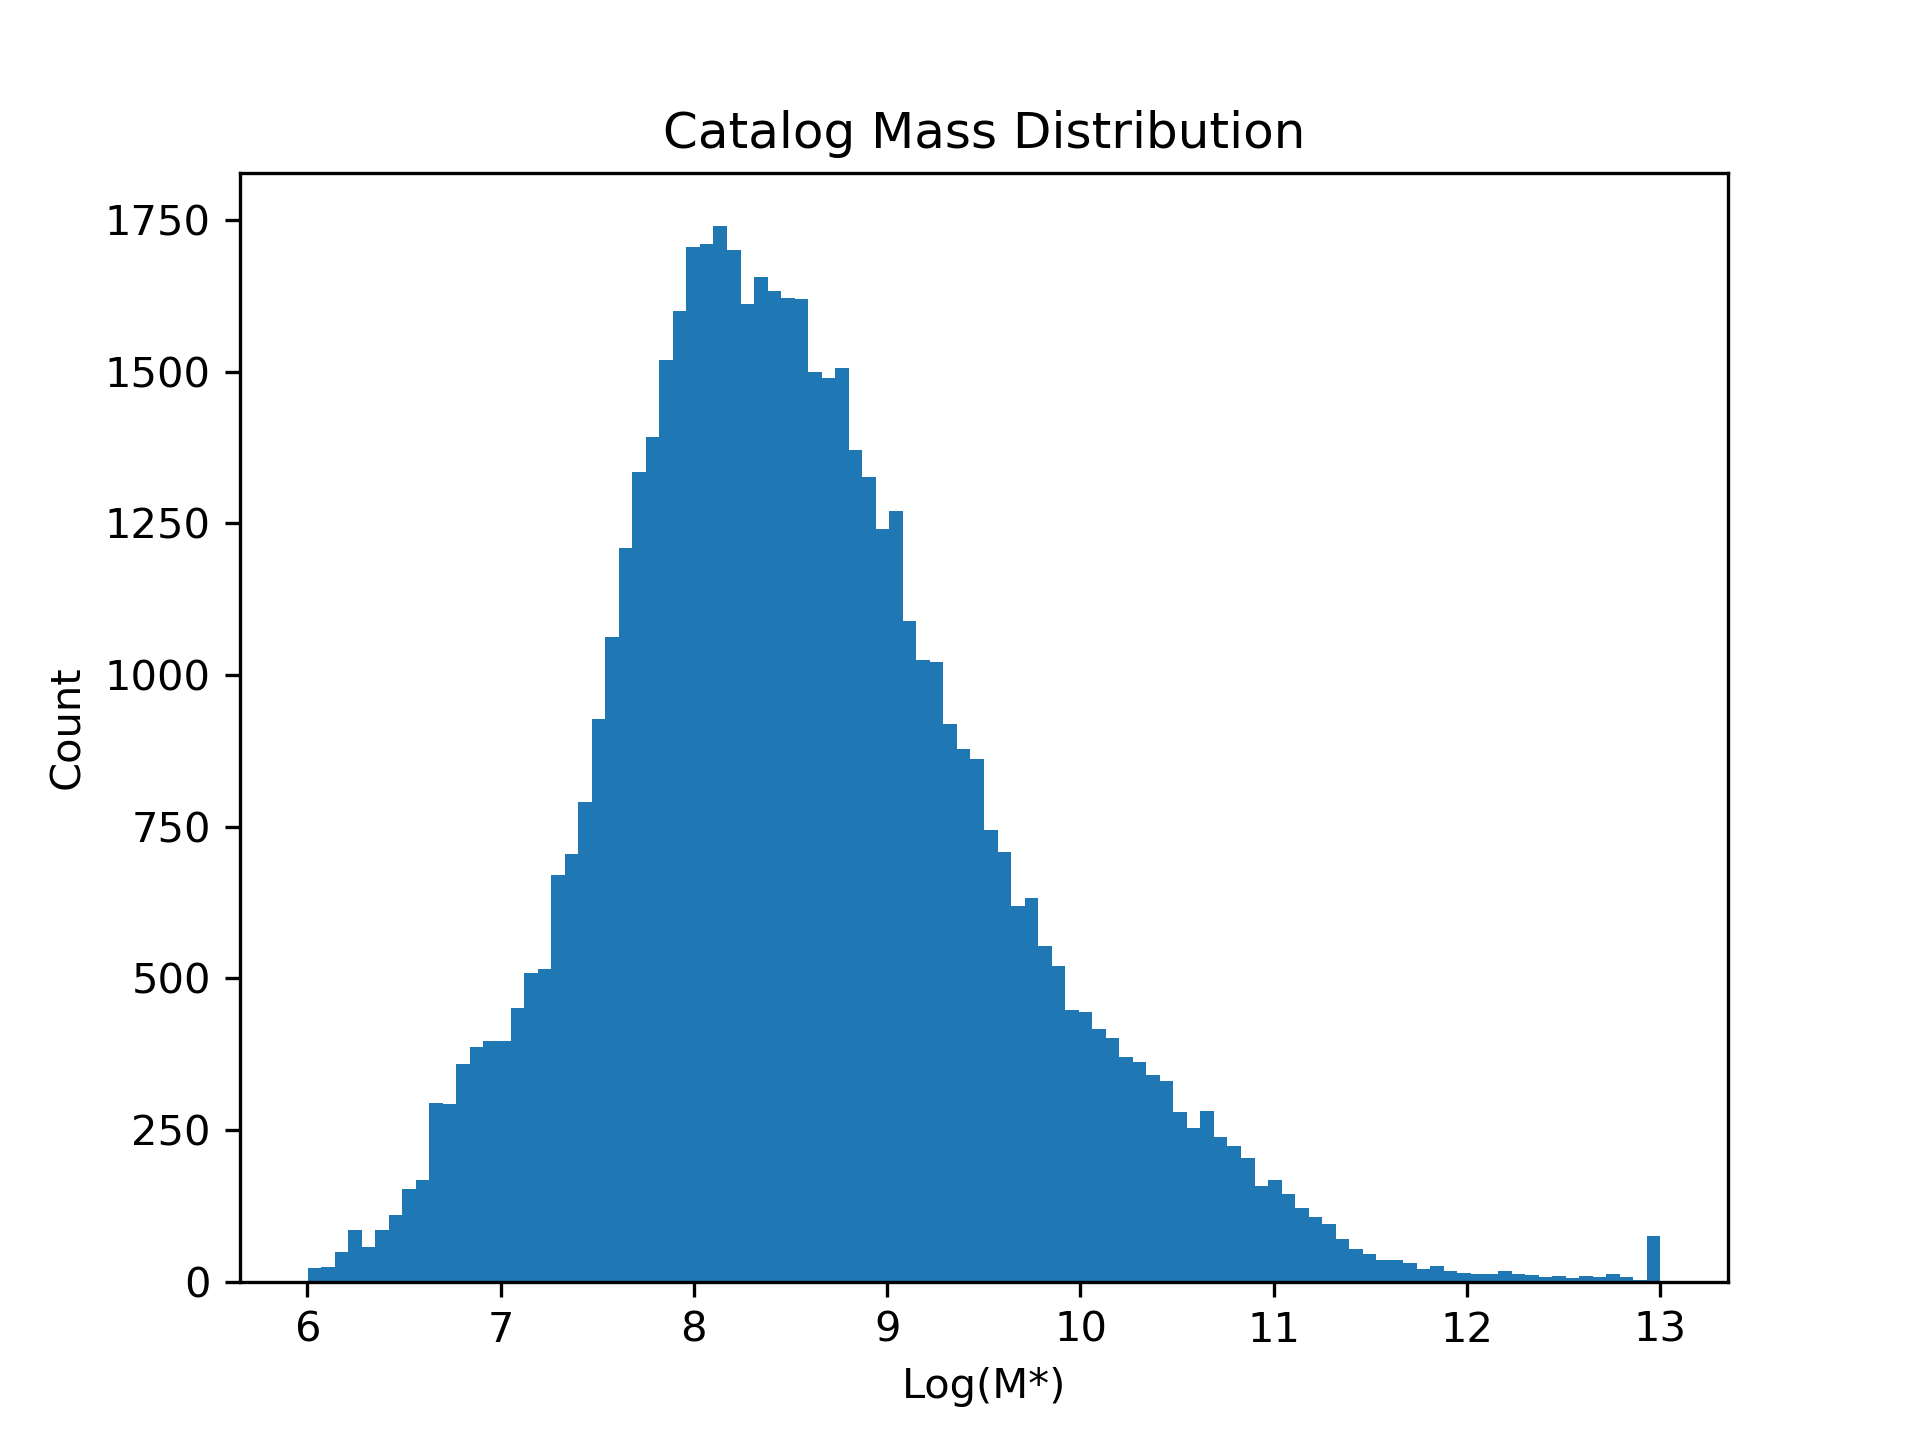
\includegraphics[width=87mm]{Survey/MAGPHYS_Mstar.png}
\caption{Distribution of stellar mass for all galaxies in the catalog. These galaxies have undergone the same quality cut as for the star-formation rate plot.}
\label{fig:MAGPHYS_Mstar}
\end{figure}

\section{The CO Emission Line Catalog}

The method for finding CO emission lines in the ALMA data cubes, computing the fidelity of the lines, cross-matching the CO emitter candidates with the galaxy catalog, and determining matches is the same process as used in the other ASPECS surveys \cite{walter2016alma, decarli2019alma, gonzalez2019alma}.

\subsection{Line Search and Fidelity}

To find possible CO emitters, a search for CO lines was done with the FindClump algorithm first described in \cite{walter2016alma}. This code searches along the spectral axis with different kernel widths in order to maximize the sensitivity to signals associated with line candidates of different intrinsic widths. The widths range from 3 spectral channels up to 19 channels, with each channel being 7.813 MHz wide, corresponding to widths of between 73.2 Km s$^{-1}$ to 463.6 Km s$^{-1}$ at 96 GHz. The data cubes are searched for lines at any spatial position and spectral coordinate, without any prior based on data from other wavelengths. This is done to minimize any bias in the selection. FindClump returns a list of potential line candidates that then have duplicates removed, which is done by grouping line candidates based on their spatial and spectral position in the cube from each group, only storing the candidate with the highest S/N \cite{walter2016alma}. This results in 11941 candidates at S/N$>$5.0, 1096 at S/N$>$5.5, 78 at S/N$>$6.0, and 6 at S/N$>$6.5. 

To get a sense of how many of these line candidates are false positives, the fidelity of the lines is then computed. To obtain the fidelity, a line search on the negative data cubes is performed using exactly the same algorithm as that used to detect lines in the positive data cubes. The negative cubes are obtained by multiplying all the values in each data cube by -1, and rerunning the line search. This catalog of negative lines is then used to compute the fidelity. The fidelity of a line at a given S/N is defined as 

$$ fideltiy(S/N) = 1 - \frac{N_{neg}(S/N)}{N_{pos}(S/N)} $$ where $N_{pos}(S/N)$ and $N_{neg}(S/N)$ are the number of positive and negative line candidates detected at that S/N and for a given line width, respectively \cite{gonzalez2019alma}.

The fidelity of the different line widths is shown in Fig. \ref{fig:Fid_map}. As can be seen, the fidelity of the lines is generally lower for narrower line widths as more independent resolution elements yield a larger probability of finding a few, high-S/N noise peaks in the cubes \cite{decarli2019alma}. The CO emission line catalog contains 16 lines at a fidelity $>$0.8, 20 at $>$0.7, 35 at $>$ 0.6, 52 at $>$ 0.5, and 69 at $>$ 0.4, and 81372 below a fidelity of 0.4. The fidelity cut used for the rest of this analysis is set at 0.6, where every given line has a 60\% chance of being a real line, and leaving us with 35 line candidates, which are listed in Table \ref{table:Catalog}.

\begin{figure}[!htbp]
\centering 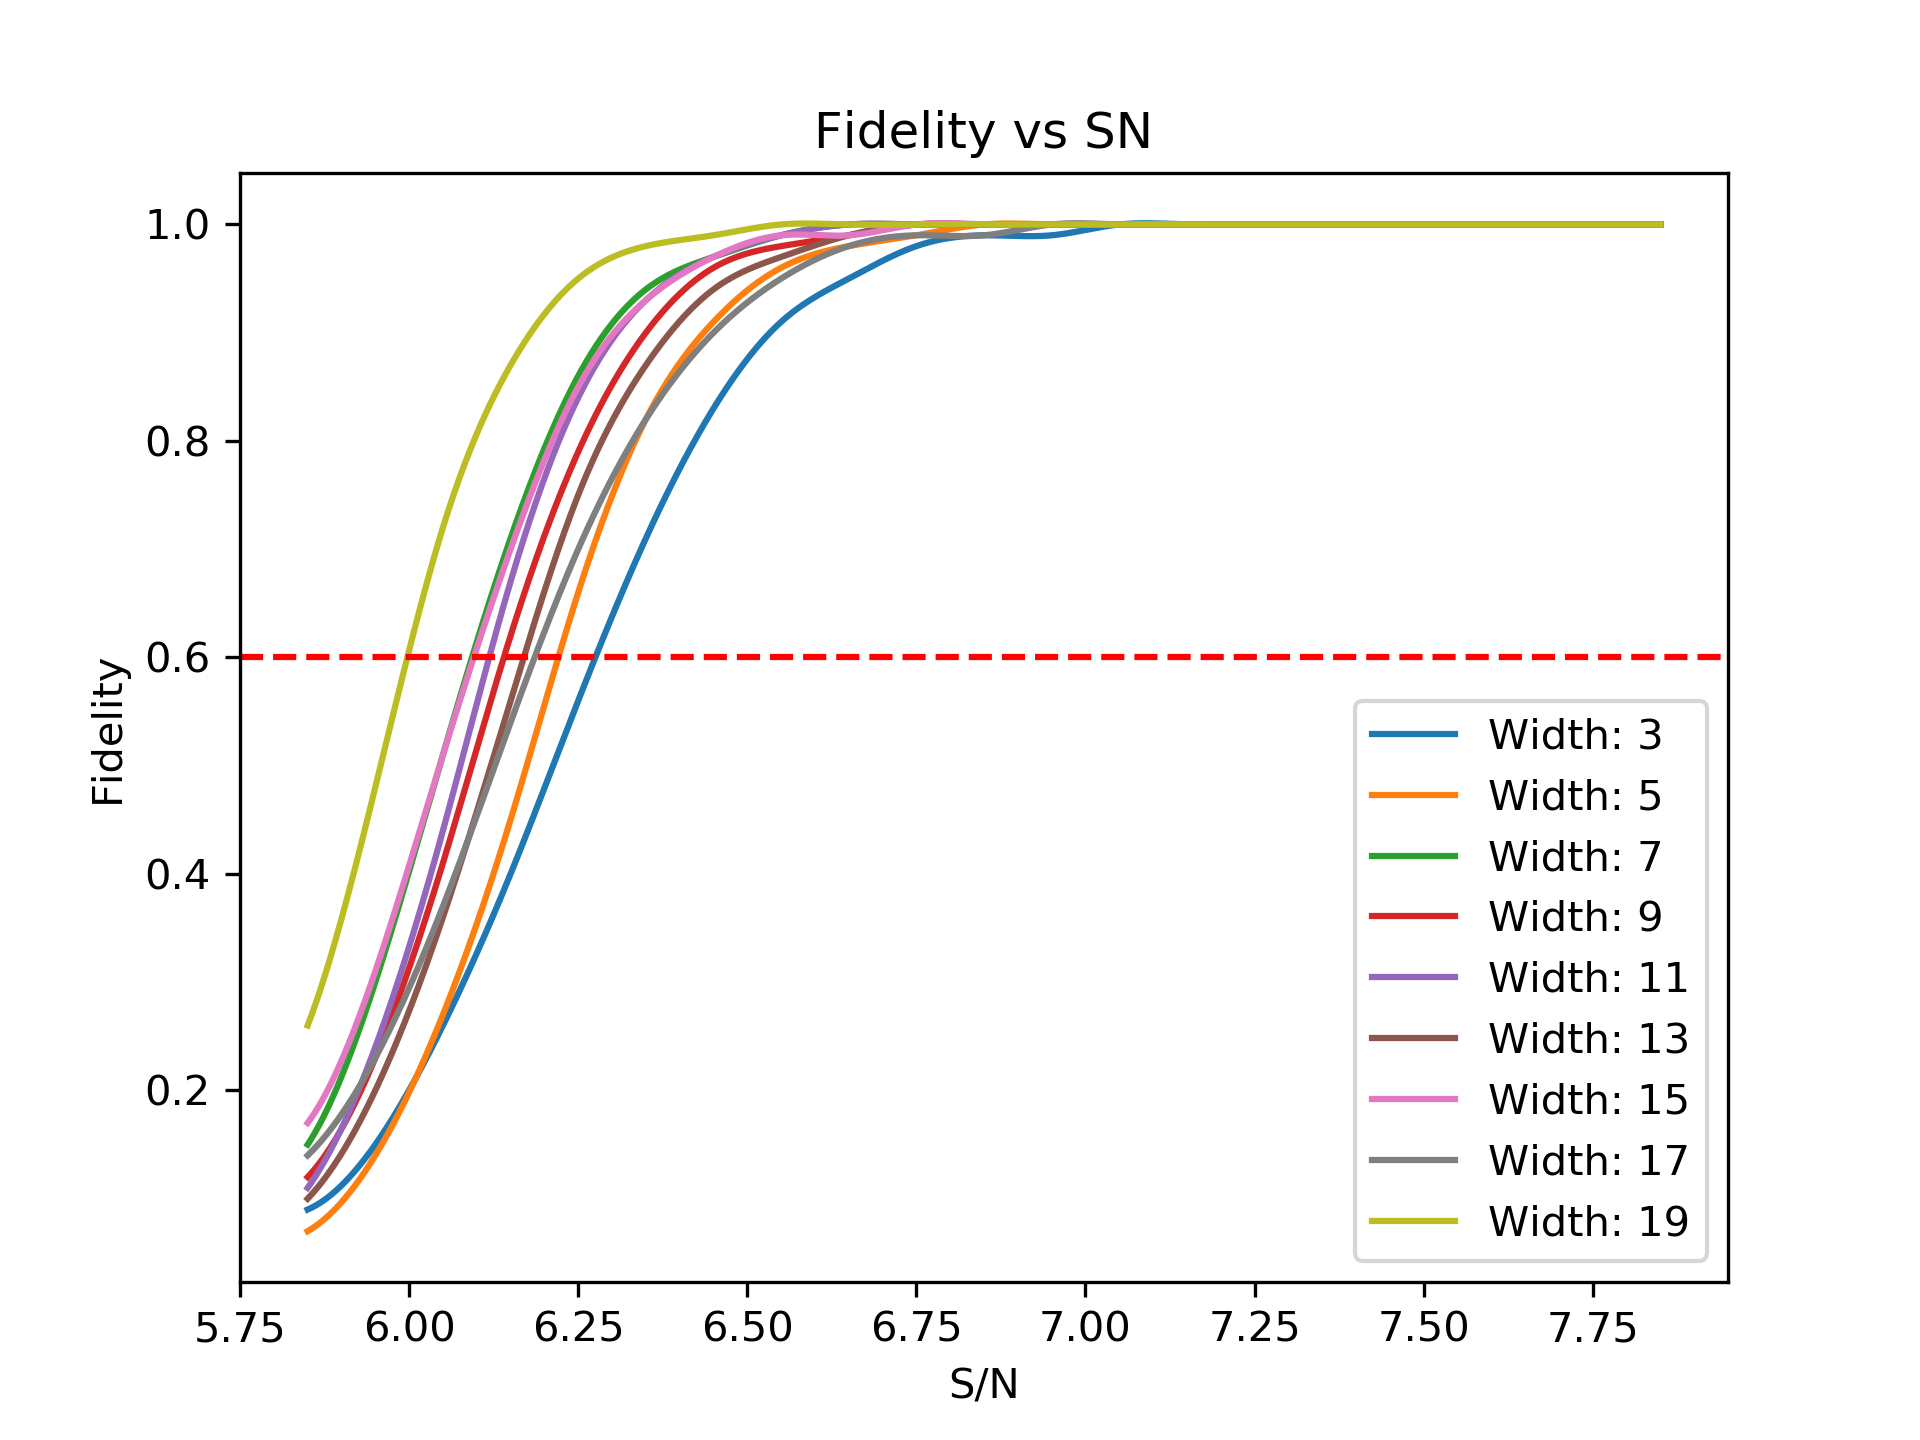
\includegraphics[width=120mm]{Fidelity_map.png}
\caption{Fidelity vs S/N for the different line widths used by FindClump. The red dotted line shows the fidelity = 0.6 cutoff used for the analysis in this report. There are a total of 35 line candidates above that cutoff.}
\label{fig:Fid_map}
\end{figure}

\subsection{Determination of the Redshift of the CO Emitters and Cross-matching with the Galaxy Catalog}

To determine the redshift of the CO emitters, we need to know the transition of the observed CO line. As shown in Table \ref{table:CO_freq}, there are multiple CO transitions which are spaced out almost equi-distant in frequency, with the CO(1-0), CO(2-1), CO(3-2), and CO(4-3) transitions having rest-frame frequencies of $\sim$115 GHz, $\sim$230 GHz, $\sim$345 GHz, and $\sim$460 GHz, respectively. This makes it difficult to determine the unique redshift for a given candidate, as multiple CO transitions could create the detected signal.

To determine the transition, and therefore the redshift, the next step after performing the line search and fidelity cut is to cross-match the CO lines to already known galaxies within the Wide ASPECS footprint. To do this, the spatial location of the line candidates is matched to galaxies that are within one arcsecond of the line candidate's location. Then, assuming that the CO line is from that matched galaxy, the CO transition is calculated. The match is only kept if the offset between the CO line's redshift and the galaxy's redshift, $\delta z$, is $|\delta z| < 0.01$ for galaxies with spectroscopic redshifts, or $|\delta z| < 0.3$ for ones with photometric redshifts. The differences in $|\delta z|$ thresholds are because spectroscopic redshifts are much more reliable and precise than photometric redshifts. 

If a line matches to more than a single galaxy then the following steps are performed to determine to which galaxy the line should be matched. The first step is to calculate the CO transition for the line assuming the line is matched to each of the galaxies. Then difference between the CO redshift and the galaxy's redshift is computed. The matched galaxy that gives the smallest $|\delta z|$ and whose redshift falls within the limits of Wide ASPECS is then saved as the matched galaxy for that line candidate. 

These counterparts provide information about the physical parameters of the line candidate. A summary of the line candidate counterparts for the fidelity $>$0.6 catalog is shown in Table \ref{table:matched_gal}. Cutouts of the three line candidates and their counterparts are shown in Figures \ref{fig:Count_One}, \ref{fig:Count_Five}, and \ref{fig:Count_Nine}. Of the counterparts, only ID.1's match has a spectroscopic redshift.

\begin{figure}[!htbp]
\centering 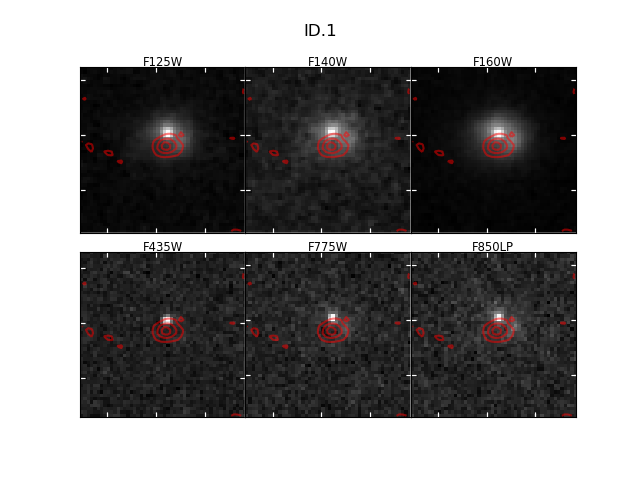
\includegraphics[width=100mm]{Matched/ASPECS_Cutout_0.png}
\caption{ID.1. Red contours signify +2$\sigma$,4$\sigma$,6$\sigma$,and 8$\sigma$. The size of the cutouts are 3x3 arcseconds. The spacing between the ticks is one arcsecond.}
\label{fig:Count_One}
\end{figure}

\begin{figure}[!htbp]
\centering 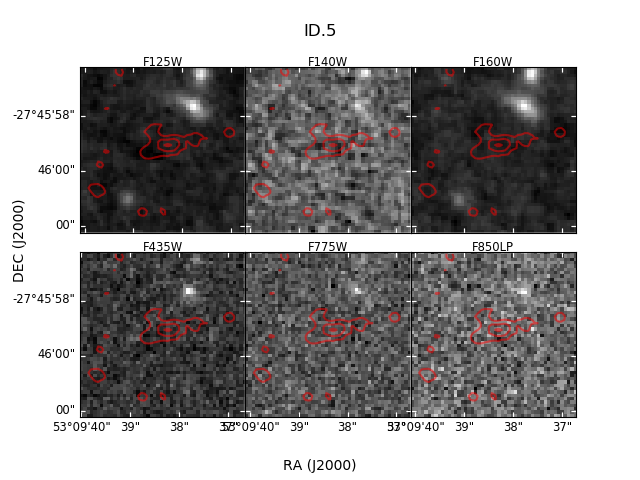
\includegraphics[width=100mm]{Matched/ASPECS_Cutout_4.png}
\caption{ID.5. Same contours and size as for Fig. \ref{fig:Count_One}. }
\label{fig:Count_Five}
\end{figure}

\begin{figure}[!htbp]
\centering 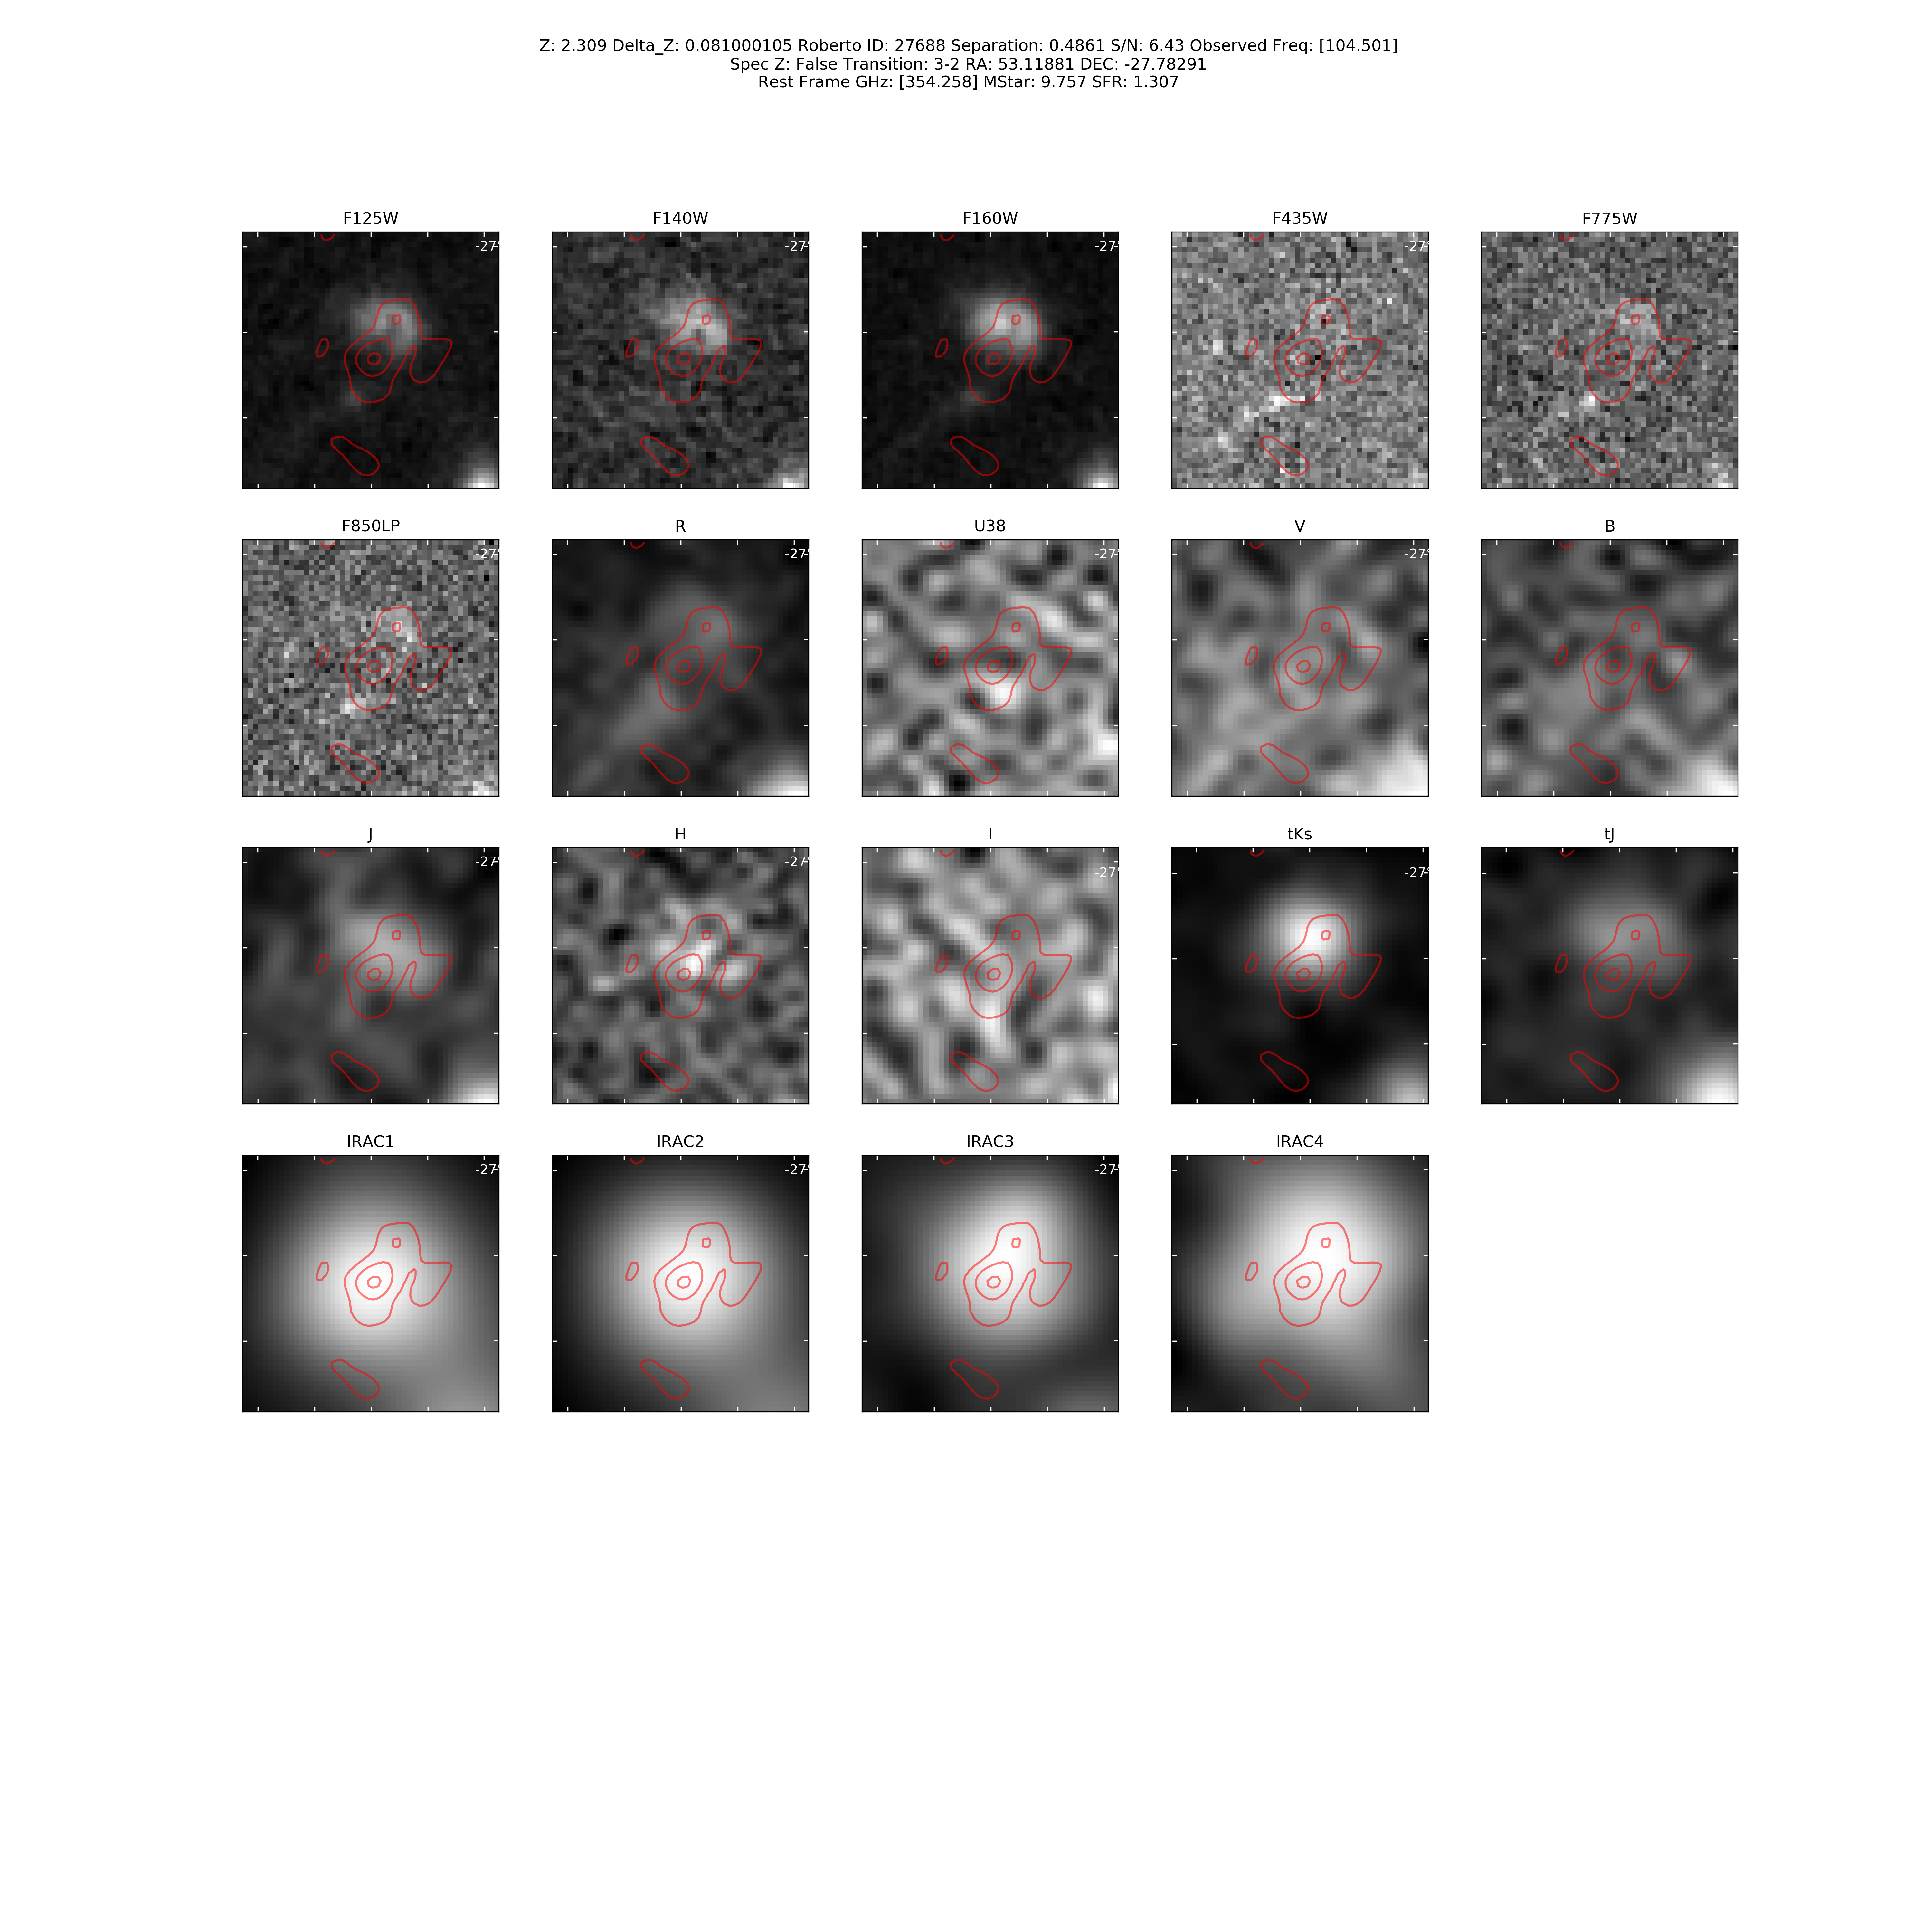
\includegraphics[width=100mm]{Matched/ASPECS_Cutout_8.png}
\caption{ID.9. Same contours and size as for Fig. \ref{fig:Count_One}.}
\label{fig:Count_Nine}
\end{figure}

If there is not a match to a galaxy in the catalog, or if the galaxy's redshift is incompatible with the CO line identification then the line identification is performed by a bootstrap method. As seen in Table \ref{table:CO_freq}, each CO transition is detectable within a certain redshift range, and that redshift range determines the volume sampled at each transition. The larger the cosmic volume probed by a given transition the more likely that an unidentified line is that transition, where the probability of a line candidate being one of CO(1-0), CO(2-1), CO(3-2), or CO(4-3) is proportional to the volume of the universe sampled in each of those transitions \cite{walter2016alma, decarli2019alma}. Once the CO line candidate's transition is determined, the redshift is computed through $ z_{CO} = \frac{Restframe_{freq}}{Obs_{freq}} - 1 $. The results of the line matching for the fidelity $>$ 0.6 sample are shown in Table \ref{table:Catalog}, and the redshift distribution of the line candidates is shown in Fig. \ref{fig:cat_red}.

\begin{table}[!htbp]
\centering
\caption{The 35 CO line candidates from the fidelity $>$ 0.6 cut.}
\begin{tabular}{ccccccccc}
ID\tablefootnote{Assigned ID for the candidate} & RA\tablefootnote{J2000 system (degrees)} & DEC\tablefootnote{J2000 system (degrees)} & $v_{CO}$\tablefootnote{Observed frequency of the source in GHz.} & CO Tran.\tablefootnote{Estimated CO transition for the line candidate. Goes from $J_{up}$ to $J_{lower}$, e.g. 3-2 is the CO(3-2) transition.} & $z_{CO}$\tablefootnote{Redshift as determined by the CO transition.} & $\delta z$\tablefootnote{Difference in redshift between the CO line transition and the galaxy the line is matched to, if there is one.} & S/N\tablefootnote{Signal-to-noise of the CO line.}& Match?\tablefootnote{If there is a match between the CO line and the galaxy catalog.} \\
\hline
ID.1 & 53.14886 & -27.82118 & 96.701 & 3-2 & 2.576 & 0.006 & 7.31 & Y \\
ID.2 & 53.19145 & -27.76985 & 91.657 & 2-1 & 1.515 & -- & 6.82 & N \\
ID.3 & 53.14138 & -27.84409 & 96.834 & 4-3 & 3.761 & -- & 6.72 & N \\
ID.4 & 53.19242 & -27.78342 & 106.72 & 3-2 & 2.24 & -- & 6.63 & N \\
ID.5 & 53.16066 & -27.76629 & 86.677 & 2-1 & 1.66 & -0.237 & 6.6 & Y \\
ID.6 & 53.16003 & -27.76258 & 103.36 & 3-2 & 2.346 & -- & 6.6 & N \\
ID.7 & 53.13447 & -27.74976 & 102.719 & 3-2 & 2.366 & -- & 6.49 & N \\
ID.8 & 53.11066 & -27.82727 & 85.654 & 3-2 & 3.037 & -- & 6.45 & N \\
ID.9 & 53.11881 & -27.78291 & 104.501 & 3-2 & 2.309 & 0.081 & 6.43 & Y \\
ID.10 & 53.13921 & -27.75352 & 86.67 & 3-2 & 2.99 & -- & 6.43 & N \\
ID.11 & 53.07696 & -27.8251 & 90.891 & 2-1 & 1.536 & -- & 6.42 & N \\
ID.12 & 53.12766 & -27.76666 & 99.553 & 4-3 & 3.631 & -- & 6.42 & N \\
ID.13 & 53.07796 & -27.80182 & 98.725 & 4-3 & 3.67 & -- & 6.36 & N \\
ID.14 & 53.13923 & -27.78228 & 94.407 & 2-1 & 1.442 & -- & 6.35 & N \\
ID.15 & 53.04266 & -27.79322 & 103.173 & 3-2 & 2.352 & -- & 6.3 & N \\
ID.16 & 53.116 & -27.84624 & 97.569 & 4-3 & 3.725 & -- & 6.29 & N \\
ID.17 & 53.09146 & -27.8497 & 106.235 & 3-2 & 2.255 & -- & 6.27 & N \\
ID.18 & 53.18748 & -27.81369 & 89.704 & 1-0 & 0.285 & -- & 6.27 & N \\
ID.19 & 53.11238 & -27.75628 & 88.735 & 3-2 & 2.897 & -- & 6.26 & N \\
ID.20 & 53.12915 & -27.79241 & 91.54 & 2-1 & 1.518 & -- & 6.22 & N \\
ID.21 & 53.1179 & -27.8184 & 92.876 & 2-1 & 1.482 & -- & 6.21 & N \\
ID.22 & 53.06549 & -27.84266 & 104.094 & 3-2 & 2.322 & -- & 6.21 & N \\
ID.23 & 53.1612 & -27.76049 & 94.618 & 2-1 & 1.437 & -- & 6.19 & N \\
ID.24 & 53.11182 & -27.82032 & 99.522 & 4-3 & 3.633 & -- & 6.19 & N \\
ID.25 & 53.07121 & -27.82724 & 88.954 & 3-2 & 2.887 & -- & 6.17 & N \\
ID.26 & 53.19977 & -27.8282 & 100.055 & 3-2 & 2.456 & -- & 6.16 & N \\
ID.27 & 53.06316 & -27.82356 & 84.623 & 3-2 & 3.086 & -- & 6.15 & N \\
ID.28 & 53.09788 & -27.76003 & 90.618 & 3-2 & 2.816 & -- & 6.13 & N \\
ID.29 & 53.16282 & -27.84445 & 90.571 & 3-2 & 2.818 & -- & 6.12 & N \\
ID.30 & 53.09665 & -27.81229 & 95.259 & 2-1 & 1.42 & -- & 6.12 & N \\
ID.31 & 53.13844 & -27.80491 & 102.376 & 3-2 & 2.378 & -- & 6.12 & N \\
ID.32 & 53.16516 & -27.82257 & 104.931 & 3-2 & 2.295 & -- & 6.11 & N \\
ID.33 & 53.19483 & -27.81481 & 98.873 & 4-3 & 3.663 & -- & 6.1 & N \\
ID.34 & 53.08948 & -27.78102 & 86.068 & 3-2 & 3.018 & -- & 6.1 & N \\
ID.35 & 53.14828 & -27.84444 & 87.302 & 3-2 & 2.961 & -- & 6.1 & N \\
\end{tabular}
\end{table}\label{table:Catalog}

\section{Physical Properties of the CO emitters}

The stellar mass versus star-formation rate is shown for the general galactic population and the 3 ASPECS counterparts in Fig. \ref{fig:Cross_match}. For comparison, the Schreiber et al. 2015 \cite{schreiber2015herschel} (as S15) and Whitaker et al. 2014 \cite{Whitaker_2014} (as W14) main sequence fits are plotted as well. As can be seen, two of the matched galaxies are above the main sequence and are massive, star-forming galaxies that are the expected type of galaxies for this survey to match to. The other galaxy is much less massive than expected. 

\begin{figure}[!htbp]
\centering 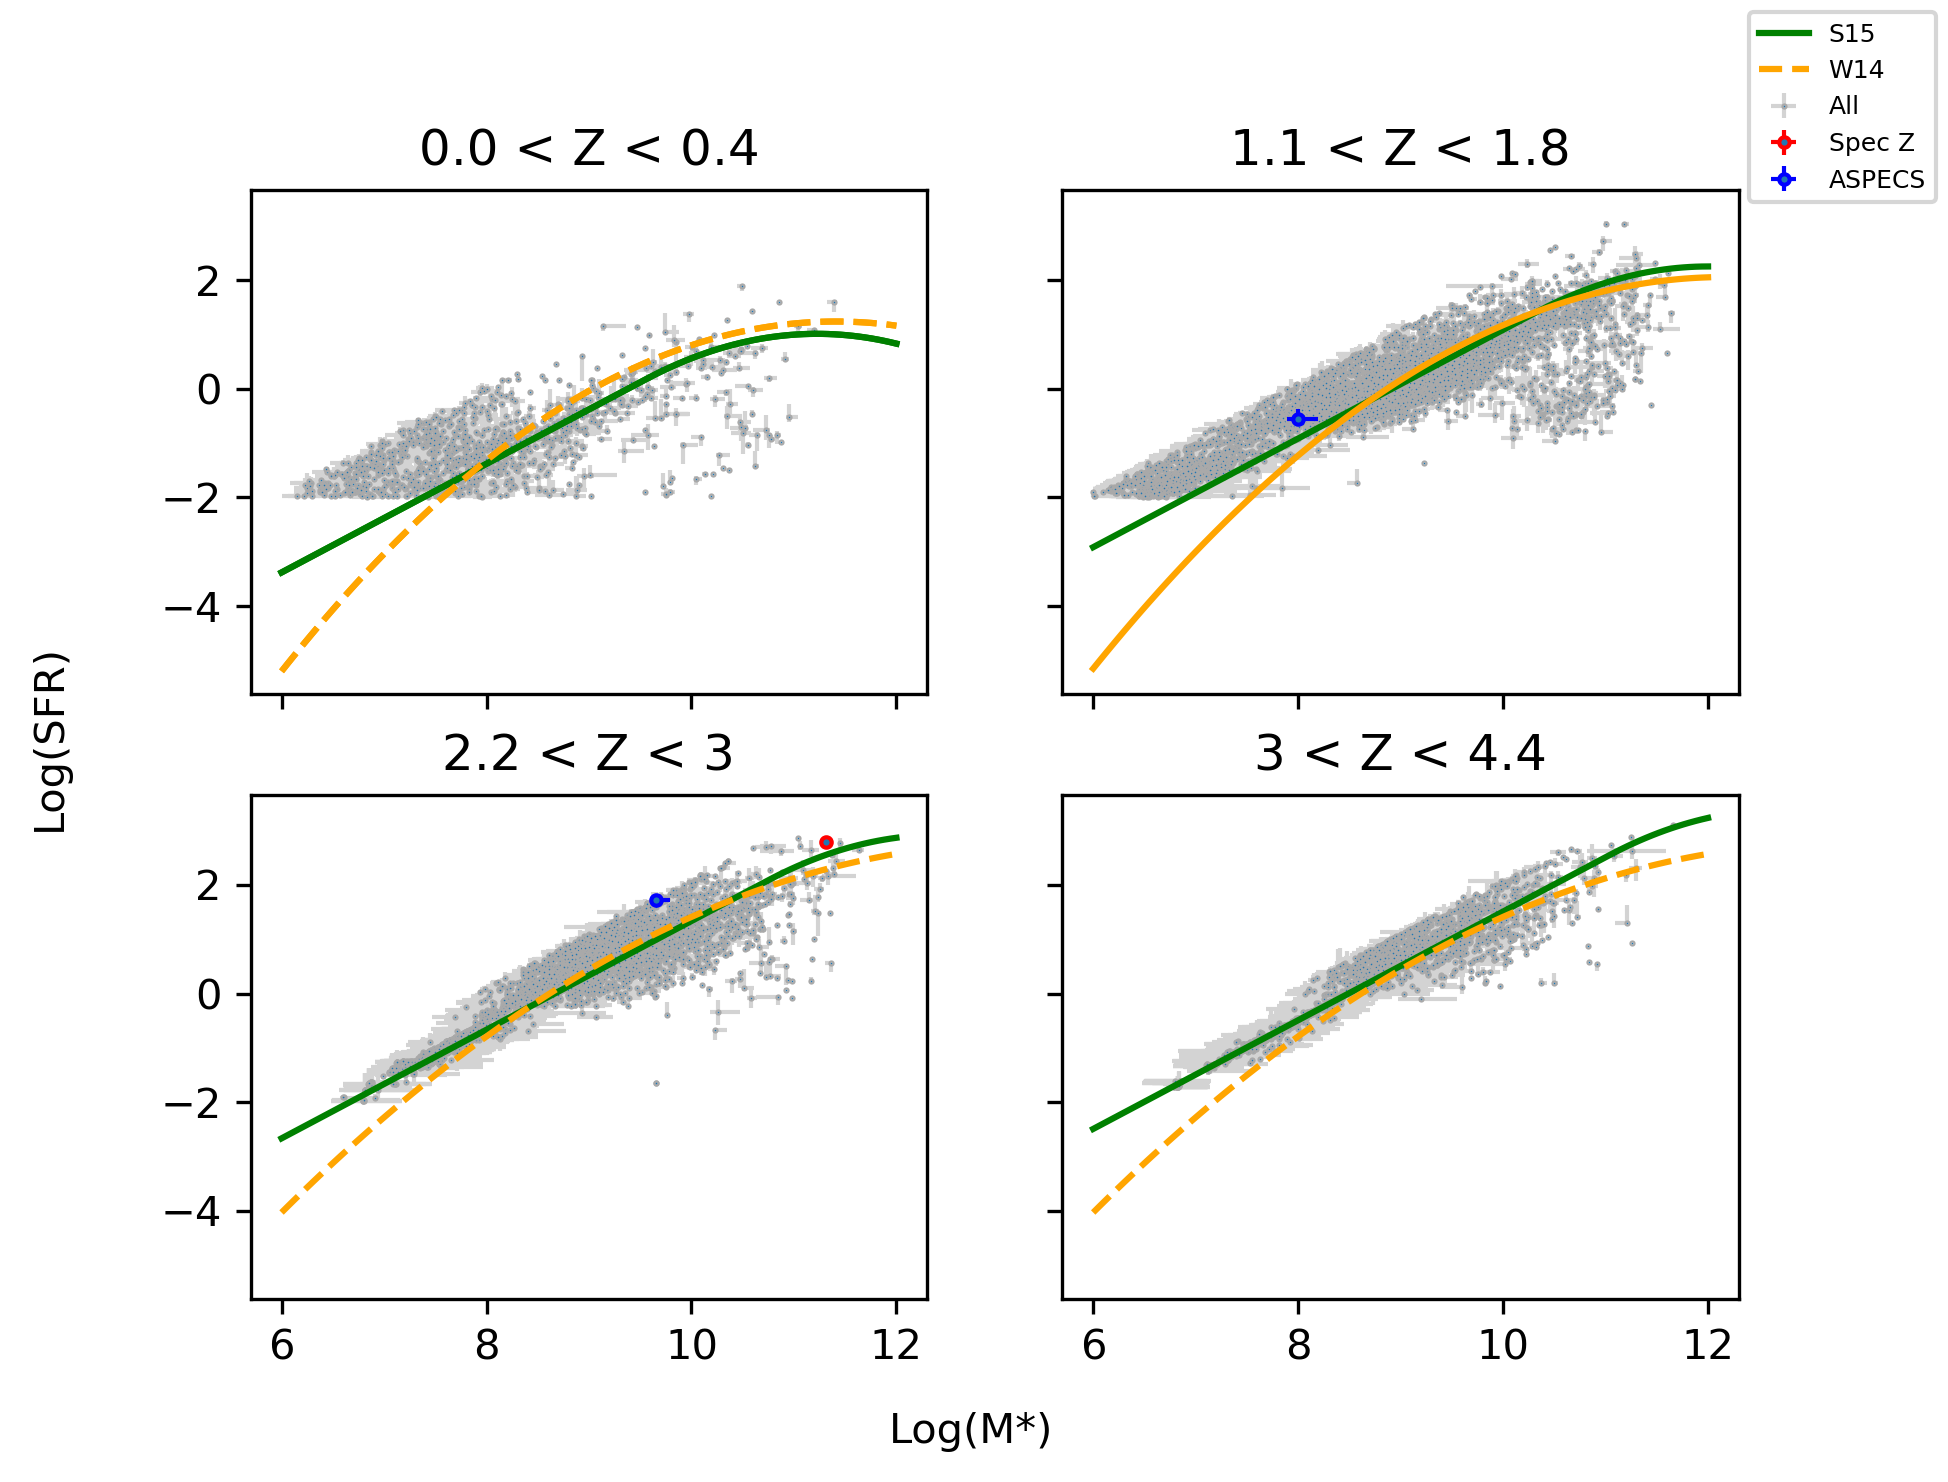
\includegraphics[width=120mm]{Survey/No_Cut_Mstar_vs_SFR_all_closest_sep_1_0_sn_fid_60.png}
\caption{Stellar mass versus star-formation rate for galaxies that the fidelity $>$ 0.6 CO line sample matched to. Red points are matched galaxies with spectroscopic redshifts, while blue points are matched galaxies with photometric redshifts. Grey points are all the galaxies in the compiled catalog from \ref{sec:ancillary}. The green lines are the galaxy main sequence fits from \cite{schreiber2015herschel}. The yellow line is from \cite{Whitaker_2014}'s galactic main sequence fit, where the solid line means it is computed within the range mentioned in the paper, while dotted means that the values are extrapolated from the paper to higher, or lower, redshifts. Two of the three matches are on the upper edge of the main sequence, while the third match has a much lower stellar mass and star-formation rate than expected for this survey. Error bars are the 16/84th percentile outputs from MAGPHYS.}
\label{fig:Cross_match}
\end{figure}

\begin{table}
\caption{This shows some of the physical parameters for the 3 matched line candidates. Sep is the separation in arcseconds between the CO line and the galaxy. $z_{catalog}$ is the master catalog's redshift for the galaxy.}
\begin{tabular}{ccccccccccccccc}
ID & Trans. & $z_{CO}$ & $z_{catalog}$ & $\delta z$ & Spec & S/N & Sep & Log(SFR) & Log(M*) \\
\hline
ID.1 & 3-2 & 2.576 & 2.582 & 0.006 & Y & 7.31 & 0.2824 & $2.782_{-0.005}^{+0.005}$ & $11.31_{-0.0}^{+0.0}$  \\
ID.5 & 2-1 & 1.66 & 1.423 & -0.237 & N & 6.6 & 0.9723 & $-0.453_{-0.115}^{+0.255}$ & $8.017_{-0.105}^{+0.175}$ \\
ID.9 & 3-2 & 2.309 & 2.39 & 0.081 & N & 6.43 & 0.4861 & $1.307_{-0.0}^{+0.0}$ & $9.757_{-0.0}^{+0.0}$ \\
\end{tabular}\label{table:matched_gal}
\end{table}

\begin{figure}[!htbp]
\centering 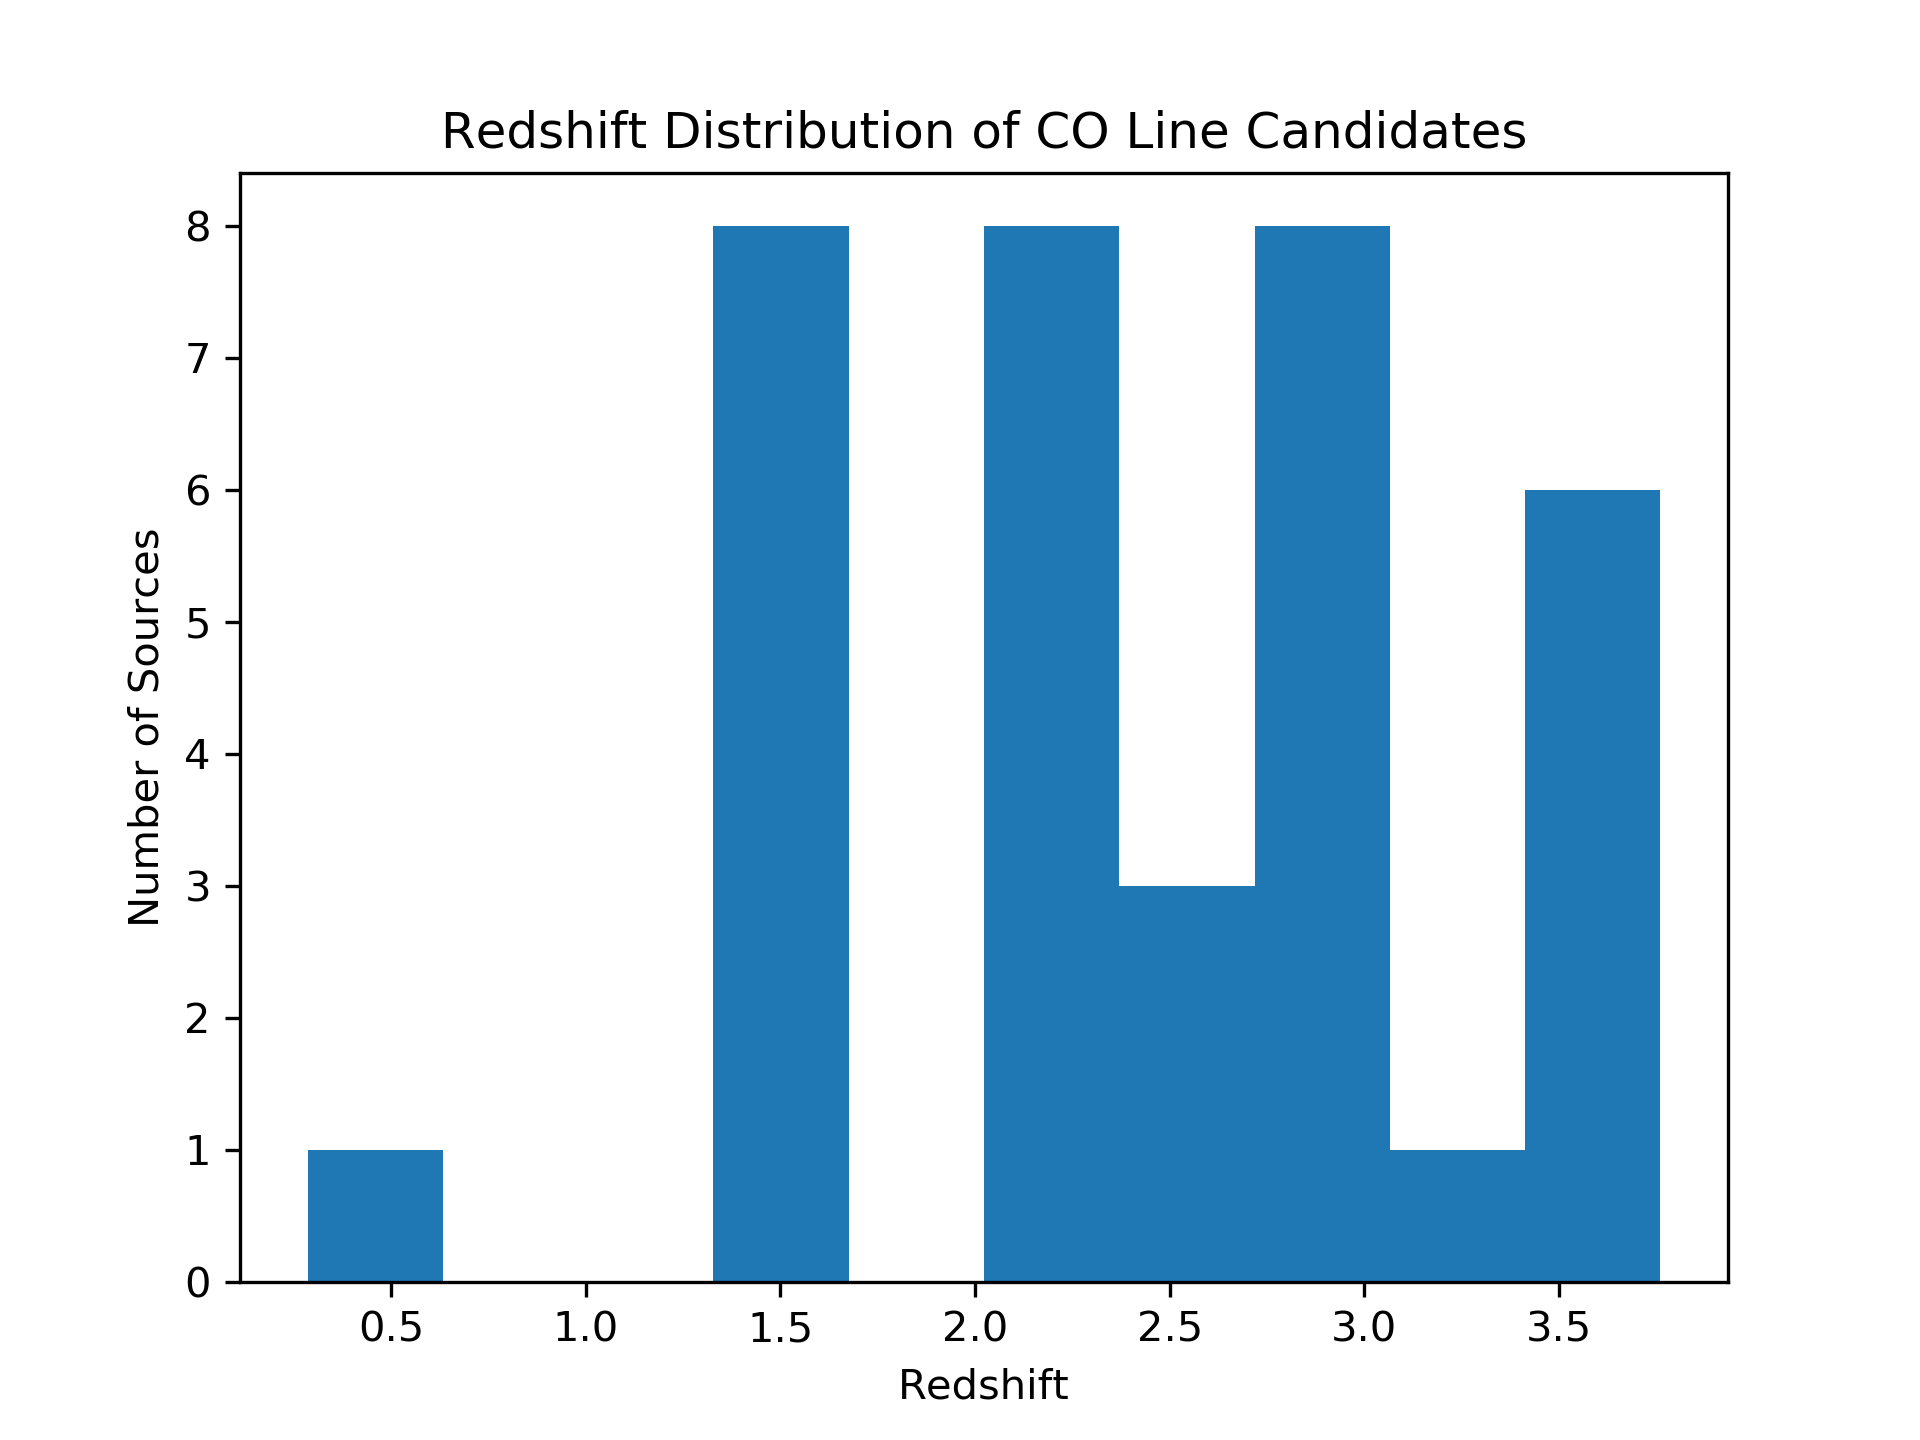
\includegraphics[width=120mm]{Survey/redshift_catalog.png}
\caption{Redshift distribution for all CO line candidate redshifts with a fidelity above 0.6, shown in Table \ref{table:Catalog}. These are the redshifts of the CO lines as determined by matching them to a CO transition, not including the redshifts of the 3 matched galaxies.}
\label{fig:cat_red}
\end{figure}

\section{Discussion}

Of the 35 line candidates chosen for the final catalog, only $\sim$9\% percent of the lines match to galaxies. Of those that do, only two matched to the most massive, most star-forming galaxies in the field. 

Possible explanations include issues with MAGPHYS' fitting of the galaxies in the catalog, as many of the galaxies seem poorly constrained. The errors in imprecise photometric redshifts could affect the estimation of the physical parameters, potentially explaining why one of the counterparts was not at the more massive end of the mass versus star-formation rate plot. The only counterpart with a spectroscopic redshift, ID.1's match, is also the counterpart with the highest stellar mass and star-formation rate, and the type of counterpart that was expected to be found in this survey.

Using a lower fidelity cut, such as a cut of $>$ 0.4, does not change the counterparts being unexpectedly composed primarily of lower stellar mass and star-forming galaxies, as seen in Fig. \ref{fig:fid_40_cross}. In fact, essentially all the extra matches from using a lower fidelity cut come from the galaxies that are the least massive and least star-forming in the field, suggesting that those matches might be spurious.

\begin{figure}[!htbp]
\centering 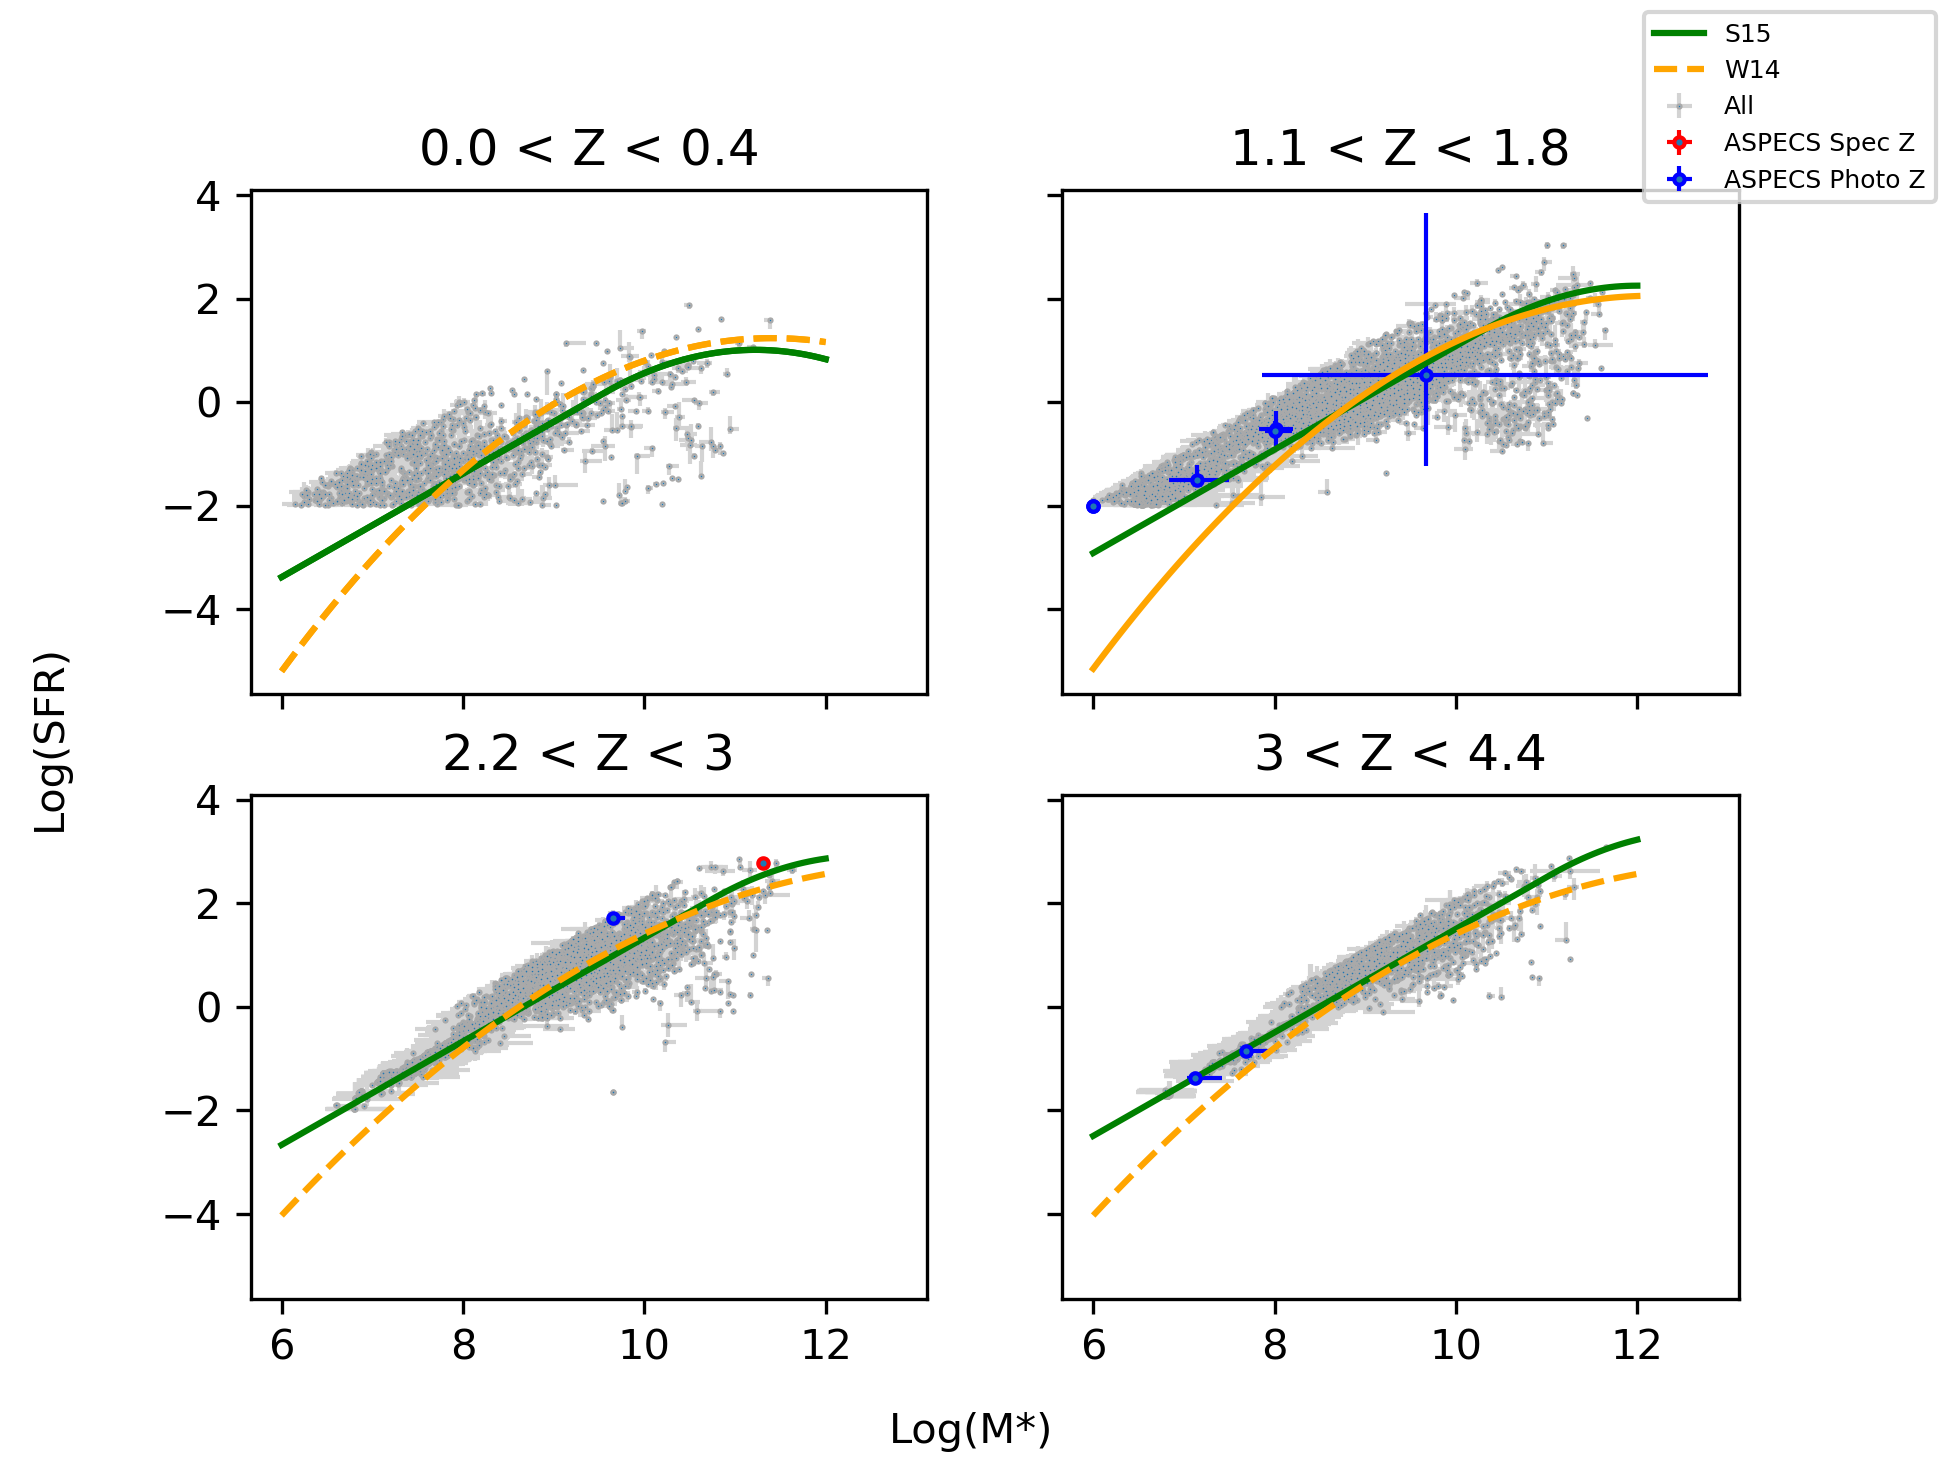
\includegraphics[width=120mm]{No_Cut_Mstar_vs_SFR_all_closest_sep_1_0_sn_fid_40.png}
\caption{Stellar mass versus star-formation rate for galaxies that the fidelity $>$ 0.4 CO line sample matched to. Red points are matched galaxies with spectroscopic redshifts, while blue points are matched galaxies with photometric redshifts. Grey points are all the galaxies in the compiled catalog from \ref{sec:ancillary}. The green lines are the galaxy main sequence fits from \cite{schreiber2015herschel}. The yellow line is from \cite{Whitaker_2014}'s galactic main sequence fit, where the solid line means it is computed within the range mentioned in the paper, while dotted means that the values are extrapolated from the paper to higher, or lower, redshifts. Two of the three matches are on the upper edge of the main sequence, the same two counterparts as for the fidelity $>$ 0.6 catalog, while the other matches have much lower stellar masses and star-formation rates than expected for this survey. Error bars are the 16/84th percentile outputs from MAGPHYS.}
\label{fig:fid_40_cross}
\end{figure}

% Physics based explanations

Other possible explanations include that the CO emitting galaxies are very dusty and optically dark, and so have not shown up in shorter wavelengths. Previous ASPECS surveys have found CO candidates without any obvious match to a previously known galaxy, along with the PdBI survey and COLDz \cite{decarli2014molecular, pavesi2018co}. This could mean that these CO lines without matches are too obscured in other wavelengths to have been detected before. As can be seen in \ref{sec:A1}, a significant number of the CO line candidates that do not match to a counterpart seem to exist in areas of the sky with very little or no other objects visible around them in optical wavelengths. 

%Try to expand a bit more this, you can also make some comments about the plot for the section fidelity cut that I suggested.

%It will maybe show more galaxies, but at lower stellar mass. You could mention that imprecise photometric errors could also affect the estimation of physical parameters (to mention a possible reason to explain why these are not at the more massive end as was expected. If you show me the plot with that cut, maybe I could give you more thoughts about what else to say.